\clearpage
\section{Constraints on proton structure}
\label{sec:protonPDFs}

By means of the strategy outlined in Sect.~\ref{sec:settings}, here we study the constraints that differential neutrino DIS
cross-section measurements at the LHC have on the quark and gluon substructure of the proton.
%
We assume an isoscalar free-nucleon target and neglect non-isoscalarity effects and nuclear modifications,
which are instead considered in Sect.~\ref{sec:nuclearPDFs}.

We present results first for the Hessian profiling of the PDF4LHC21 combination,
and second for the inclusion in the Monte Carlo fit NNPDF4.0.
%
We study the stability of the results with respect to the inclusion of systematic uncertainties
and  charm-tagged events, as well to the availability of outgoing lepton-charge separation.
%
We compare the impact of four of the experiments considered in Sect.~\ref{sec:dis_pseudodata}:
FASER$\nu$ and SND@LHC (LHC Run III) with FASER$\nu$2 and AdvSND (HL-LHC).

\subsection{Hessian profiling of PDF4LHC21}
\label{sec:pdf4lhc21}

For the Hessian profiling studies based on the procedure of Sect.~\ref{sec:profiling}, the prior PDF set is taken to
be PDF4LHC21 NNLO, a Monte Carlo combination~\cite{Watt:2012tq,Carrazza:2015hva} of three global PDF sets (CT18~\cite{Hou:2019efy},
MSHT20~\cite{Bailey:2020ooq}, and NNPDF3.1~\cite{NNPDF:2017mvq}).
%
The Hessian representations of PDF4LHC21 are obtained by means of the methodology developed in~\cite{Gao:2013bia,Carrazza:2015aoa}.
%
Being based on the combination of three modern global PDF fits, PDF4LHC21 provides a robust estimate
of  current uncertainties associated to our understanding of proton PDFs.
%
We profile PDF4LHC21 with various sets of LHC neutrino DIS projections in order to assess the stability
of the results with respect to its different inputs, such as charm-tagged structure functions.
%
A tolerance of $T = \sqrt{\Delta \chi^2}=3$ is adopted, corresponding to the average tolerance
used in the CT18 and MSHT20 Hessian determinations.
%
The consistent perturbative accuracy of the prior PDF set and the theoretical calculations entering
the pseudo-data generation is always accounted for.

For the baseline results, we consider FASER$\nu$2 operative for the full duration
of the HL-LHC data-taking period.
%
Both inclusive and charm-tagged structure functions enter the profiling,
and outgoing lepton charge-separation is assumed.
%
Fig.~\ref{fig:profiling_syst} displays the
fractional uncertainties   (68\% confidence level) at $Q^2 = 10^4 \, \textrm{GeV}^2$ 
for the up and down valence quarks, gluon, total quark singlet, and total strangeness PDFs
in PDF4LHC21 compared to the results of its profiling with the FASER$\nu$2 projections.
%
For the latter, we consider two scenarios: first where the covariance matrix includes
only statistical errors, and second with experimental systematic
errors added in quadrature to the statistical ones.
%
Note that the residual shift in central values, which depends on the arbitrary fluctuations
entering the pseudo-data generation, is not displayed.

%%%%%%%%%%%%%%%%%%%%%%%%%%%%%%%%%%%%%%%%%%%%%%%%%%%%%%%%%%%%%%%%%%%%%%%%
\begin{figure}[t]
\centering
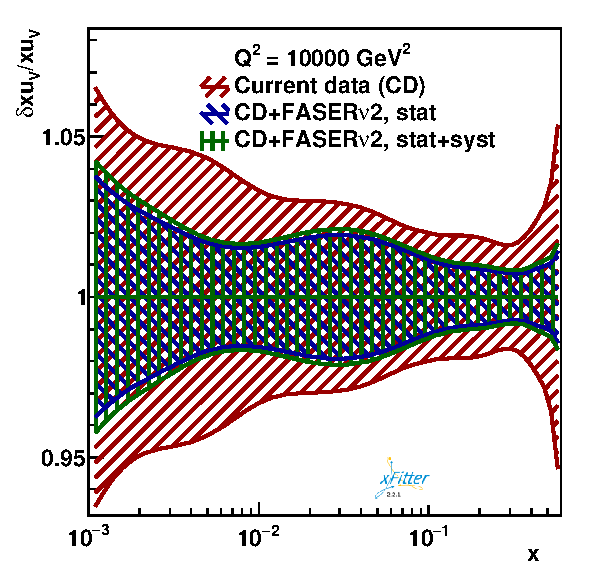
\includegraphics[width=0.32\textwidth]{plots/proton_fasernu2/inclusive+charm_chargediscrimination/syst_FASERv2_q2_10000_pdf_uv_ratio.pdf}
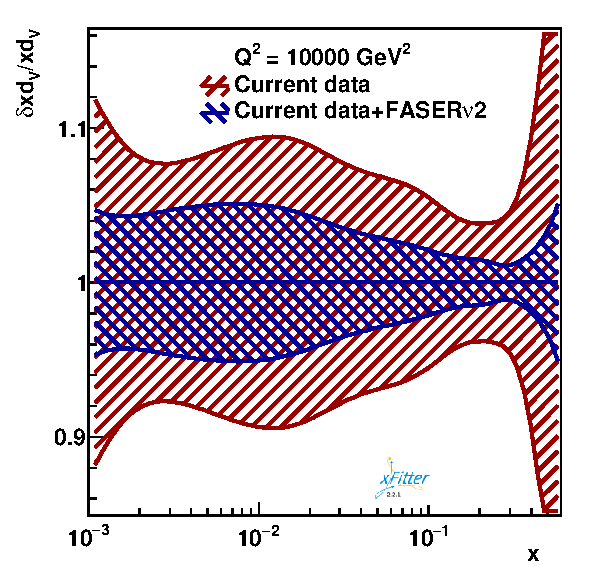
\includegraphics[width=0.32\textwidth]{plots/proton_fasernu2/inclusive+charm_chargediscrimination/syst_FASERv2_q2_10000_pdf_dv_ratio.pdf}
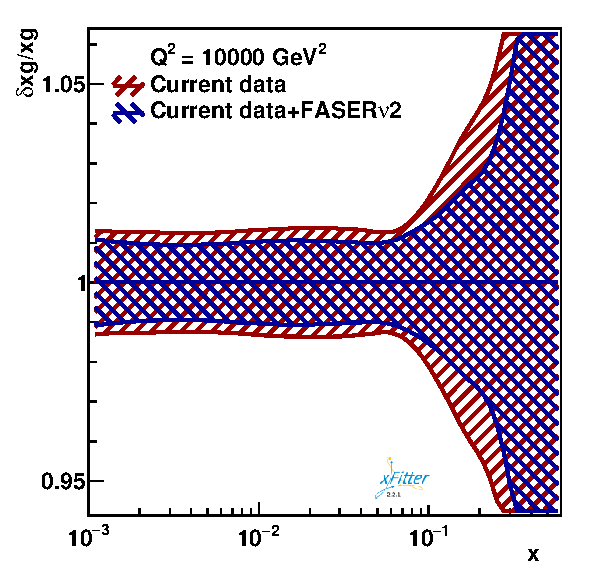
\includegraphics[width=0.32\textwidth]{plots/proton_fasernu2/inclusive+charm_chargediscrimination/syst_FASERv2_q2_10000_pdf_g_ratio.pdf}\\
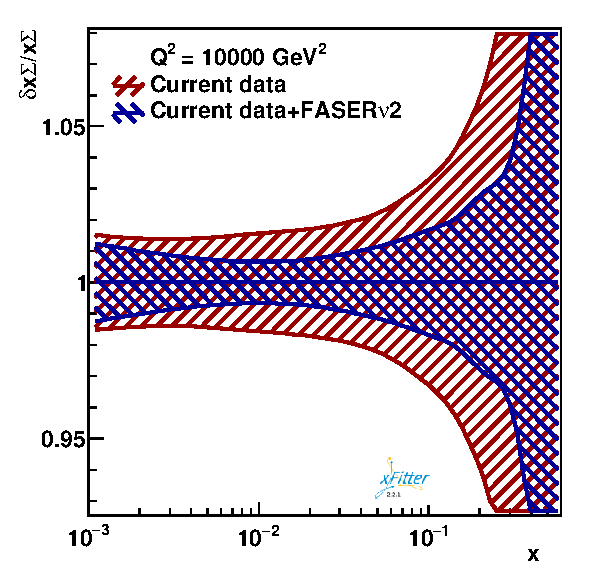
\includegraphics[width=0.32\textwidth]{plots/proton_fasernu2/inclusive+charm_chargediscrimination/syst_FASERv2_q2_10000_pdf_Sea_ratio.pdf}
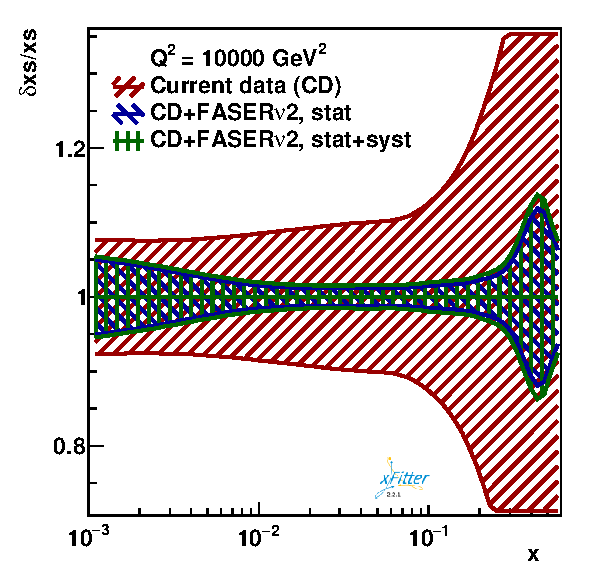
\includegraphics[width=0.32\textwidth]{plots/proton_fasernu2/inclusive+charm_chargediscrimination/syst_FASERv2_q2_10000_pdf_s_ratio.pdf}
\caption{
The fractional uncertainties   (68\% confidence level) at $Q^2 = 10^4 \, \textrm{GeV}^2$ 
for the up and down valence quarks, gluon, total quark singlet, and total strangeness PDFs
in PDF4LHC21 compared to the results of its profiling with the FASER$\nu$2
DIS projections.
%
In the latter case, we consider both only statistical errors and statistical and systematic
errors added in quadrature.
%
The FASER$\nu$2 dataset used here accounts for both  inclusive and charm-tagged structure functions
as well as for outgoing lepton charge-separation.
%
}
\label{fig:profiling_syst}
\end{figure}
%%%%%%%%%%%%%%%%%%%%%%%%%%%%%%%%%%%%%%%%%%%%%%%%%%%%%%%%%%%%%%%%%%%%%%%%

Inspection of Fig.~\ref{fig:profiling_syst} reveals that measurement of DIS structure
functions at FASER$\nu$2 impose stringent constraints on the quark PDFs, while leaving
the gluon PDF essentially unaffected.
%
As expected for a neutrino scattering experiment, its impact is most marked for
those PDF combinations sensitive to quark flavour separation such as $u_V$, $d_V$, and
$s^+$.
%
The reduction of PDF uncertainties is particularly significant for the total strangeness PDF,
as  consequence of the inclusion of charm-tagged structure functions in the fit as we demonstrate below.
%
Crucially, one finds that for the assumptions on the systematic uncertainties
discussed in Sect~\ref{sec:dis_pseudodata}, the PDF sensitivity is only marginally degraded
as compared to the case in which systematic errors are neglected.
%
This result is consistent with Fig.~\ref{fig:percentage_uncertainties_overview}, showing
how in most bins systematic and statistical errors are of similar magnitude.

In the following we consider the stability of the results in Fig.~\ref{fig:profiling_baseline}
with respect to the chosen experiment and integrated luminosity, the modelling of systematic
uncertainties, being able to identify or not charm production, and being able to tell part outgoing
charged leptons from anti-leptons.


%
Fig.~\ref{fig:profiling_charm} displays a comparison of the baseline LHC neutrino dataset with the results
of profiling without the charm production structure functions. 
Particularly, the constraints on the $s$ PDF are observed to become more stringent 
by virtue of the contribution of the charm production structure functions.

%%%%%%%%%%%%%%%%%%%%%%%%%%%%%%%%%%%%%%%%%%%%%%%%%%%%%%%%%%%%%%%%%%%%%%%%
\begin{figure}[t]
\centering
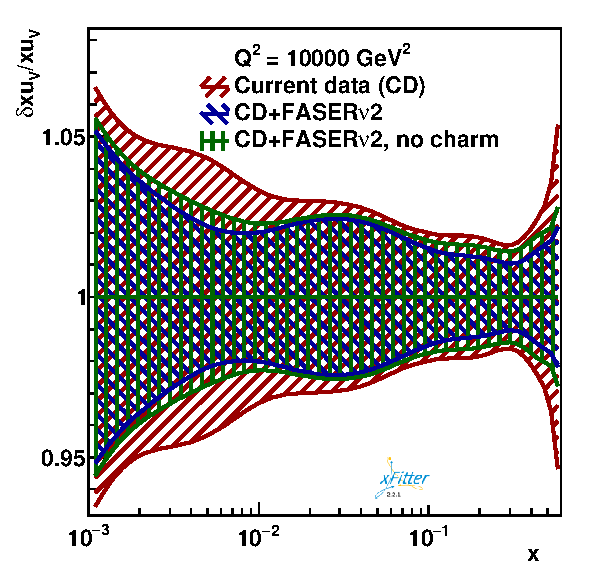
\includegraphics[width=0.32\textwidth]{plots/proton_fasernu2/inclusive-only_vs_inclusive+charm/statOnly_FASERv2_q2_10000_pdf_uv_ratio.pdf}
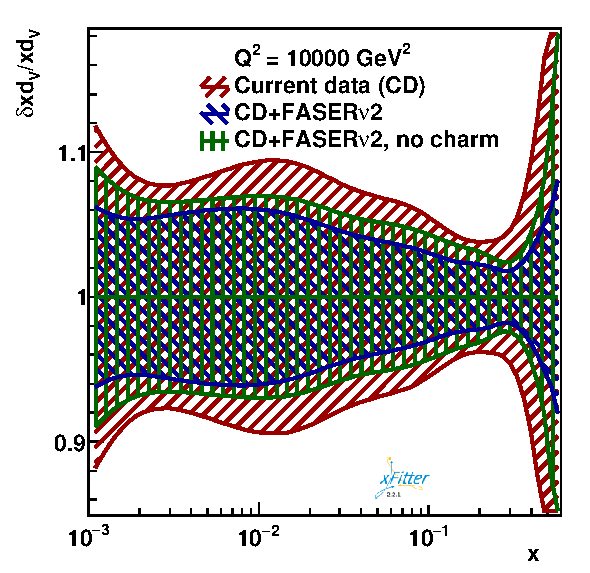
\includegraphics[width=0.32\textwidth]{plots/proton_fasernu2/inclusive-only_vs_inclusive+charm/statOnly_FASERv2_q2_10000_pdf_dv_ratio.pdf}
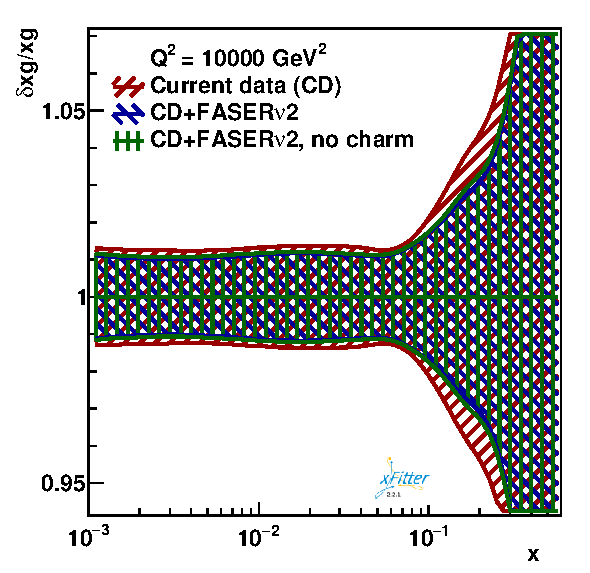
\includegraphics[width=0.32\textwidth]{plots/proton_fasernu2/inclusive-only_vs_inclusive+charm/statOnly_FASERv2_q2_10000_pdf_g_ratio.pdf}\\
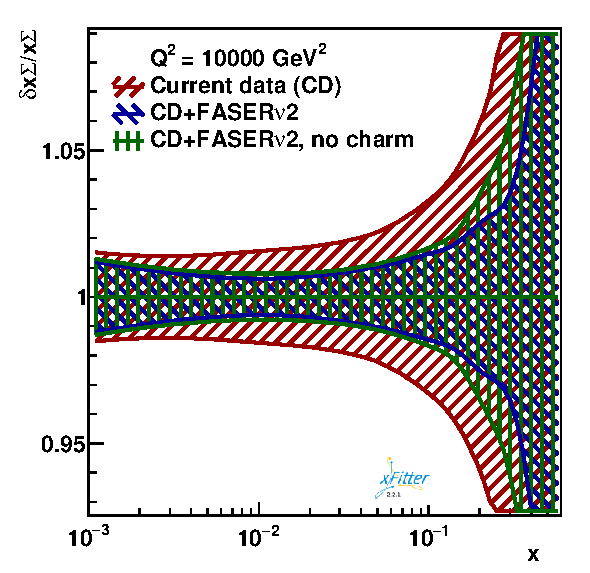
\includegraphics[width=0.32\textwidth]{plots/proton_fasernu2/inclusive-only_vs_inclusive+charm/statOnly_FASERv2_q2_10000_pdf_Sea_ratio.pdf}
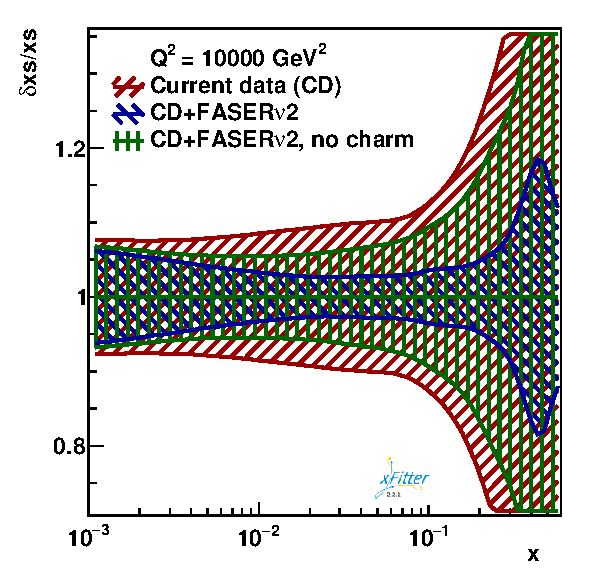
\includegraphics[width=0.32\textwidth]{plots/proton_fasernu2/inclusive-only_vs_inclusive+charm/statOnly_FASERv2_q2_10000_pdf_s_ratio.pdf}
\caption{Same as Fig.~\ref{fig:profiling_syst}, now assessing the impact of FASER$\nu$2 structure functions
once charm-tagged measurements are removed.
%
In both cases, the covariance matrix accounts for systematic uncertainties.
}
\label{fig:profiling_charm}
\end{figure}
%%%%%%%%%%%%%%%%%%%%%%%%%%%%%%%%%%%%%%%%%%%%%%%%%%%%%%%%%%%%%%%%%%%%%%%%

%
Fig.~\ref{fig:profiling_nochargediscrimination} compares the baseline LHC neutrino dataset with the results
of a profiling without allowing for the possibility of outgoing lepton charge separation.
%%%%%%%%%%%%%%%%%%%%%%%%%%%%%%%%%%%%%%%%%%%%%%%%%%%%%%%%%%%%%%%%%%%%%%%%
\begin{figure}[t]
\centering
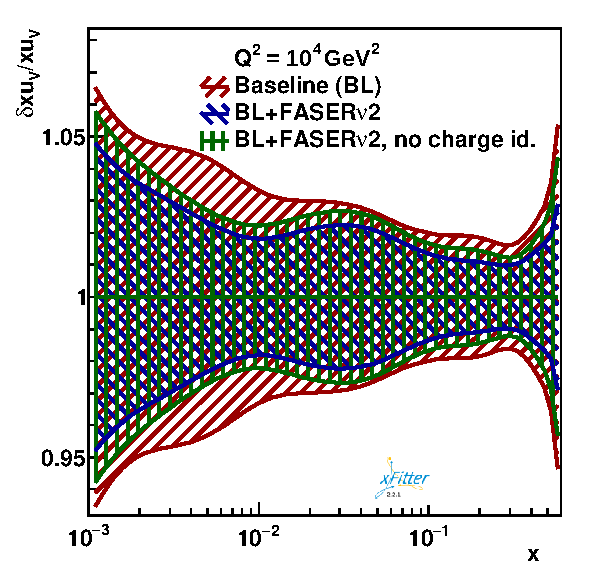
\includegraphics[width=0.32\textwidth]{plots/proton_fasernu2/nochargediscrimination/statOnly_FASERv2_q2_10000_pdf_uv_ratio.pdf}
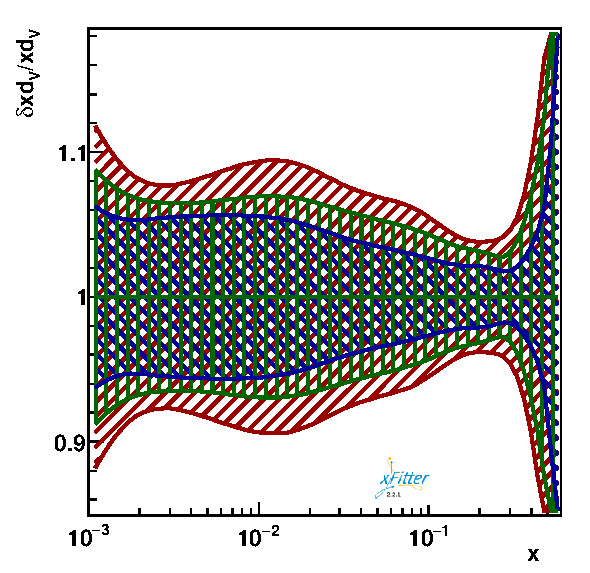
\includegraphics[width=0.32\textwidth]{plots/proton_fasernu2/nochargediscrimination/statOnly_FASERv2_q2_10000_pdf_dv_ratio.pdf}
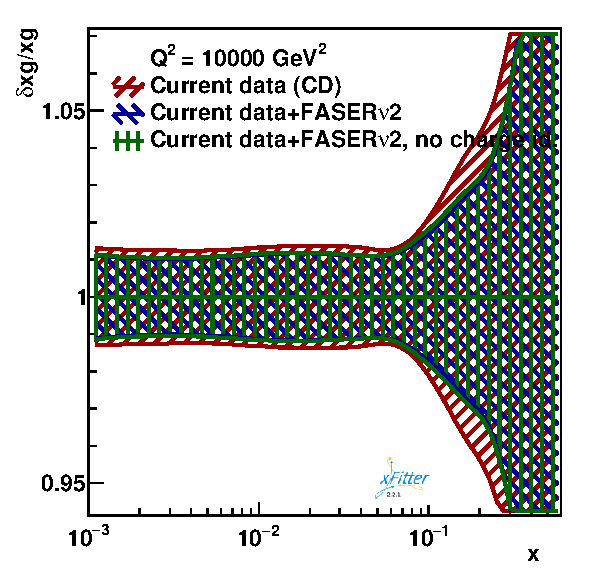
\includegraphics[width=0.32\textwidth]{plots/proton_fasernu2/nochargediscrimination/statOnly_FASERv2_q2_10000_pdf_g_ratio.pdf}\\
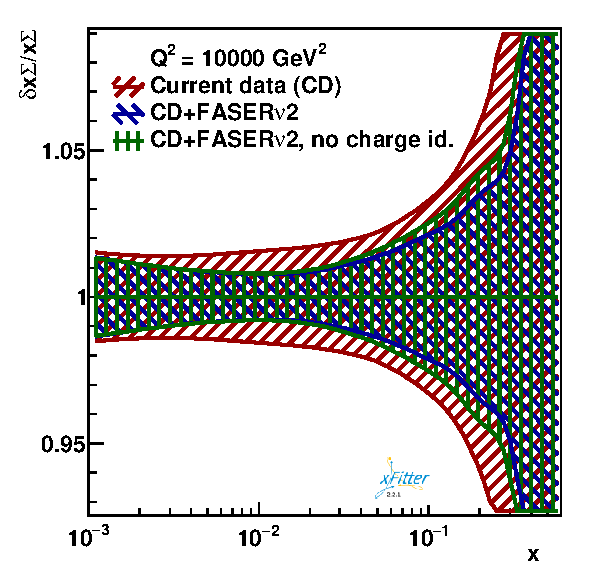
\includegraphics[width=0.32\textwidth]{plots/proton_fasernu2/nochargediscrimination/statOnly_FASERv2_q2_10000_pdf_Sea_ratio.pdf}
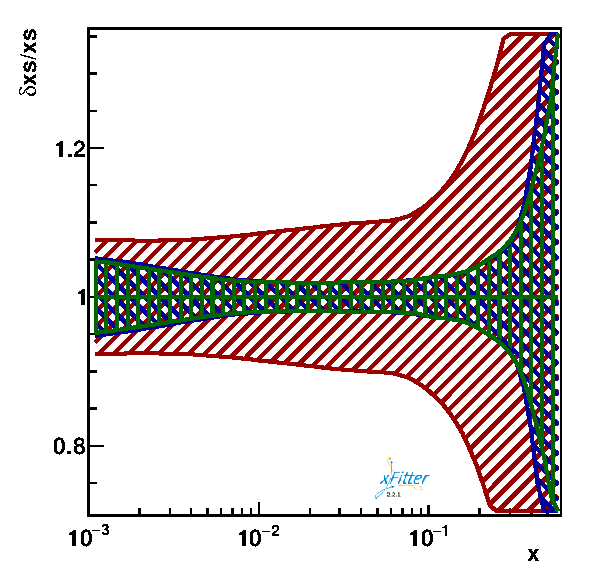
\includegraphics[width=0.32\textwidth]{plots/proton_fasernu2/nochargediscrimination/statOnly_FASERv2_q2_10000_pdf_s_ratio.pdf}
\caption{
Same as Fig.~\ref{fig:profiling_syst}, now assessing the impact of that being unable to identify
the charge of the outgoing lepton would have on the FASER$\nu$2 reach on the proton PDFs.
%
In both cases, the covariance matrix accounts for systematic uncertainties.
}
\label{fig:profiling_nochargediscrimination}
\end{figure}
%%%%%%%%%%%%%%%%%%%%%%%%%%%%%%%%%%%%%%%%%%%%%%%%%%%%%%%%%%%%%%%%%%%%%%%%


{\bf add discussion of experiment sensitivity}
%
Same as Fig.~\ref{fig:profiling_syst} comparing FASER$\nu$2 with AdvSND and with FASER$\nu$.



\subsection{Impact on NNPDF4.0}
\label{sec:nnpdf40}

Selection of the {\sc\small xFitter} results for the NNPDF case.
